\documentclass[12pt]{exam}
\usepackage{amsthm}
\usepackage{bm}
\usepackage{libertine}
\usepackage[utf8]{inputenc}
\usepackage[margin=0.5in]{geometry}
\usepackage{amsmath,amssymb}
\usepackage{multicol}
\usepackage[shortlabels]{enumitem}
\usepackage{siunitx}
\usepackage{physics}
\usepackage{booktabs}
\usepackage{graphicx}
\usepackage{pgfplots}
\usepackage{listings}
\usepackage{tikz}
\usepackage{tikz-3dplot}

\bmdefine{\ii}{i}
\bmdefine{\jj}{j}
\bmdefine{\kk}{k}
\newcommand{\te}{\theta}
\newcommand{\cC}{\mathcal{C}}
\newcommand{\word}[1]{\quad\text{#1}\quad}

\pgfplotsset{width=10cm,compat=1.9}
\usepgfplotslibrary{external}
\tikzexternalize
% Keep the small vector diagrams embedded; no external images or shell escape.
\tikzexternaldisable
\tikzset{
  quizregion/.style={fill=blue!9,draw=black,line width=0.7pt},
  quizaxis/.style={->,line width=0.6pt},
  quizslice/.style={very thick,blue!65!black},
  every picture/.style={font=\small}
}

\newcommand{\class}{Math 261-001}
\newcommand{\examnum}{Quiz 4 Solutions}
\newcommand{\examdate}{September 25}

\begin{document}
\pagestyle{plain}
\thispagestyle{empty}

\noindent
\textbf{\class}\\
\textbf{\examnum}, \textbf{\examdate}

\vspace{10pt}
\small
\begin{enumerate}

\item \textbf{Final answer:}
\[
  \boxed{\int_0^1\int_{y^2}^{2-y}f(x,y)\,dx\,dy}.
\]

The two original regions have bounds
\[
  D_1:\quad
  \left\{
  \begin{aligned}
    &0\leq x\leq1,\\
    &0\leq y\leq\sqrt{x}
  \end{aligned}
  \right.
  \qquad
  D_2:\quad
  \left\{
  \begin{aligned}
    &1\leq x\leq2,\\
    &0\leq y\leq2-x.
  \end{aligned}
  \right.
\]
They meet along $x=1$, and the curves meet at $(1,1)$.
A horizontal slice joins $[y^2,1]$ and $[1,2-y]$, giving the combined bounds
\[
  \left\{
  \begin{aligned}
    &0\leq y\leq1,\\
    &y^2\leq x\leq2-y.
  \end{aligned}
  \right.
\]

\begin{center}
\begin{minipage}[t]{0.46\linewidth}
\centering
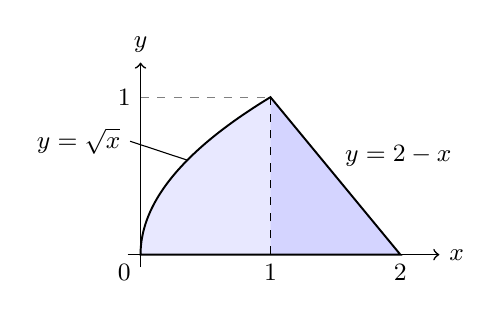
\begin{tikzpicture}[x=1.65cm,y=2cm]
  \path[fill=blue!9] (0,0)--(1,0)--(1,1)
    --plot[domain=1:0,samples=60,variable=\t] ({\t*\t},\t)--cycle;
  \path[fill=blue!17] (1,0)--(2,0)--(1,1)--cycle;
  \draw[line width=0.7pt] (0,0)--(2,0)--(1,1)
    --plot[domain=1:0,samples=60,variable=\t] ({\t*\t},\t)--cycle;
  \draw[dashed] (1,0)--(1,1);
  \draw[dashed,gray] (0,1)--(1,1);
  \draw[quizaxis] (-0.10,0)--(2.3,0) node[right] {$x$};
  \draw[quizaxis] (0,-0.08)--(0,1.22) node[above] {$y$};
  \node[below left] at (0,0) {$0$};
  \node[below] at (1,0) {$1$};
  \node[below] at (2,0) {$2$};
  \node[left] at (0,1) {$1$};
  \draw[thin] (0.36,0.6)--(-0.08,0.72) node[left] {$y=\sqrt{x}$};
  \node[above right] at (1.5,0.5) {$y=2-x$};
  %\draw[quizslice] (0.36,0)--(0.36,0.6) (1.5,0)--(1.5,0.5);
  %\fill[blue!65!black] (0.36,0) circle (1pt) (0.36,0.6) circle (1pt)
  %  (1.5,0) circle (1pt) (1.5,0.5) circle (1pt);
\end{tikzpicture}

\textit{Original: two regions split at $x=1$.}
\end{minipage}\hfill
\begin{minipage}[t]{0.46\linewidth}
\centering
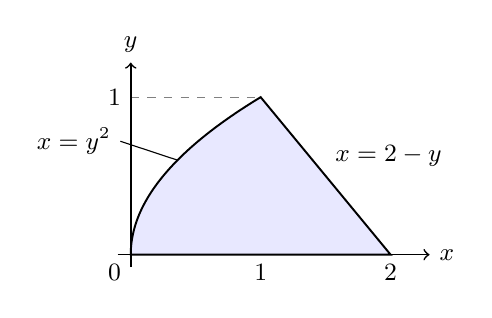
\begin{tikzpicture}[x=1.65cm,y=2cm]
  \path[quizregion] (0,0)--(2,0)--(1,1)
    --plot[domain=1:0,samples=60,variable=\t] ({\t*\t},\t)--cycle;
  \draw[dashed,gray] (0,1)--(1,1);
  \draw[quizaxis] (-0.10,0)--(2.3,0) node[right] {$x$};
  \draw[quizaxis] (0,-0.08)--(0,1.22) node[above] {$y$};
  \node[below left] at (0,0) {$0$};
  \node[below] at (1,0) {$1$};
  \node[below] at (2,0) {$2$};
  \node[left] at (0,1) {$1$};
  \draw[thin] (0.36,0.6)--(-0.08,0.72) node[left] {$x=y^2$};
  \node[above right] at (1.5,0.5) {$x=2-y$};
  %\draw[quizslice] (0.25,0.5)--(1.5,0.5);
  %\fill[blue!65!black] (0.25,0.5) circle (1pt) (1.5,0.5) circle (1pt);
\end{tikzpicture}

\textit{Reversed: one slice, $y^2\leq x\leq2-y$.}
\end{minipage}
\end{center}

As a check, setting $f=1$ gives area $\tfrac23+\tfrac12=\tfrac76$ in the
original order, and $\int_0^1(2-y-y^2)\,dy=\tfrac76$ in the new order.

\item \textbf{Final answer:}
\[
  \boxed{M=\int_0^2\int_0^{2-x}\int_0^{4-y^2}(1+z)\,dz\,dy\,dx}.
\]

The triangular $xy$-projection $D$ and the solid $E$ have bounds
\[
  D:\quad
  \left\{
  \begin{aligned}
    &x\geq0,\\
    &y\geq0,\\
    &x+y\leq2
  \end{aligned}
  \right.
  \qquad
  E:\quad
  \left\{
  \begin{aligned}
    &0\leq x\leq2,\\
    &0\leq y\leq2-x,\\
    &0\leq z\leq4-y^2.
  \end{aligned}
  \right.
\]
Above each base point, the height is $4-y^2$. Multiplying the volume element
by the density $\rho=1+z$ gives the mass integral. No evaluation is required.

\begin{center}
\begin{minipage}[c]{0.56\linewidth}
\centering
% Oblique projection of the exact patch (s(2-t),t,4-t^2).
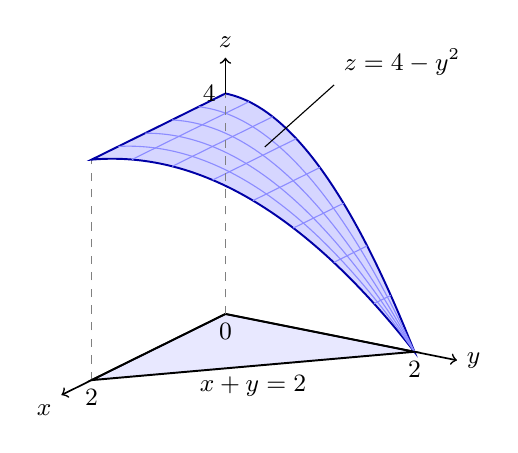
\begin{tikzpicture}[
  x={(-0.85cm,-0.42cm)},y={(1.2cm,-0.24cm)},z={(0cm,0.7cm)}]
  \path[quizregion] (0,0,0)--(2,0,0)--(0,2,0)--cycle;
  \draw[dashed,gray] (0,0,0)--(0,0,4) (2,0,0)--(2,0,4);
  \path[fill=blue!16,draw=blue!65!black,line width=0.7pt]
    (0,0,4)--(2,0,4)
    --plot[domain=0:2,samples=60,variable=\t]
      ({2-\t},{\t},{4-\t*\t})
    --plot[domain=2:0,samples=60,variable=\t]
      (0,{\t},{4-\t*\t})--cycle;
  % Constant-y rulings and constant-s curves stay on the triangular patch.
  \foreach \t in {0.25,0.5,...,1.75} {
    \draw[blue!45,thin]
      (0,\t,{4-\t*\t})--({2-\t},\t,{4-\t*\t});
  }
  \foreach \s in {0.2,0.4,0.6,0.8} {
    \draw[blue!45,thin] plot[domain=0:2,samples=60,variable=\t]
      ({\s*(2-\t)},{\t},{4-\t*\t});
  }
  \draw[quizaxis] (0,0,0)--(2.45,0,0) node[below left] {$x$};
  \draw[quizaxis] (0,0,0)--(0,2.45,0) node[right] {$y$};
  \draw[dashed,gray] (0,0,0)--(0,0,4);
  \draw[quizaxis] (0,0,4)--(0,0,4.65) node[above] {$z$};
  \node[below] at (0,0,0) {$0$};
  \node[below] at (2,0,0) {$2$};
  \node[below] at (0,2,0) {$2$};
  \node[left] at (0,0,4) {$4$};
  \draw[thin] (0.4,0.7,{4-0.7*0.7})--(0,1.15,4.55)
    node[above right] {$z=4-y^2$};
  \node[below,sloped] at (1,1,0) {$x+y=2$};
\end{tikzpicture}

\textit{The surface $(x,y,4-y^2)$ above the triangular base.}
\end{minipage}\hfill
\begin{minipage}[c]{0.40\linewidth}
\centering
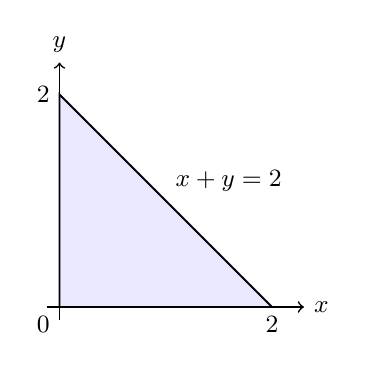
\begin{tikzpicture}[x=1.35cm,y=1.35cm]
  \path[quizregion] (0,0)--(2,0)--(0,2)--cycle;
  \draw[quizaxis] (-0.12,0)--(2.3,0) node[right] {$x$};
  \draw[quizaxis] (0,-0.12)--(0,2.3) node[above] {$y$};
  \node[below left] at (0,0) {$0$};
  \node[below] at (2,0) {$2$};
  \node[left] at (0,2) {$2$};
  \node[above right] at (1,1) {$x+y=2$};
  %\draw[quizslice] (0.75,0)--(0.75,1.25);
  %\fill[blue!65!black] (0.75,0) circle (1pt) (0.75,1.25) circle (1pt);
\end{tikzpicture}

\textit{$xy$-projection: $0\leq y\leq2-x$.}
\end{minipage}
\end{center}
Using $0\leq x,y\leq2$ and $0\leq z\leq4$ instead would integrate over a
larger rectangular box.

\newpage

\item \textbf{Final answer:}
\[
  \boxed{\int_0^1\int_0^y h(x,y)\,dx\,dy
  +\int_1^2\int_0^{2-y}h(x,y)\,dx\,dy}.
\]

The original bounds are
\[
  \left\{
  \begin{aligned}
    &0\leq x\leq1,\\
    &x\leq y\leq2-x.
  \end{aligned}
  \right.
\]
They describe the triangle with vertices $(0,0)$, $(0,2)$, and $(1,1)$.
For fixed $y$, both $x\leq y$ and $x\leq2-y$ must hold. Horizontal slices
therefore split at $y=1$, giving
\[
  \left\{
  \begin{aligned}
    &0\leq y\leq1,\\
    &0\leq x\leq y
  \end{aligned}
  \right.
  \qquad\text{or}\qquad
  \left\{
  \begin{aligned}
    &1\leq y\leq2,\\
    &0\leq x\leq2-y.
  \end{aligned}
  \right.
\]

\begin{center}
\begin{minipage}[t]{0.46\linewidth}
\centering
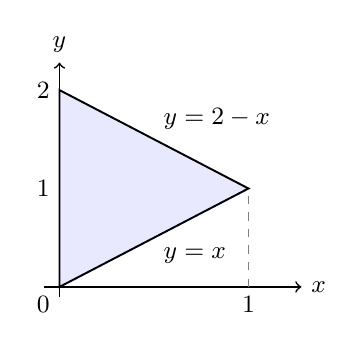
\begin{tikzpicture}[x=2.4cm,y=1.25cm]
  \path[quizregion] (0,0)--(1,1)--(0,2)--cycle;
  \draw[quizaxis] (-0.08,0)--(1.28,0) node[right] {$x$};
  \draw[quizaxis] (0,-0.10)--(0,2.28) node[above] {$y$};
  \draw[dashed,gray] (1,0)--(1,1);
  \node[below left] at (0,0) {$0$};
  \node[below] at (1,0) {$1$};
  \node[left] at (0,1) {$1$};
  \node[left] at (0,2) {$2$};
  \node[below right] at (0.5,0.5) {$y=x$};
  \node[above right] at (0.5,1.5) {$y=2-x$};
  %\draw[quizslice] (0.4,0.4)--(0.4,1.6);
  %\fill[blue!65!black] (0.4,0.4) circle (1pt) (0.4,1.6) circle (1pt);
\end{tikzpicture}

\textit{Original: $x\leq y\leq2-x$.}
\end{minipage}\hfill
\begin{minipage}[t]{0.46\linewidth}
\centering
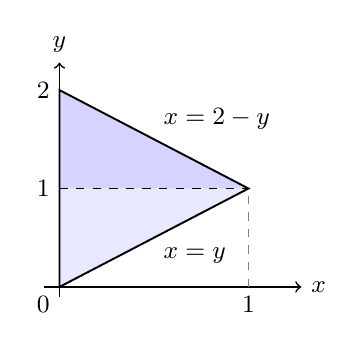
\begin{tikzpicture}[x=2.4cm,y=1.25cm]
  \path[fill=blue!9] (0,0)--(1,1)--(0,1)--cycle;
  \path[fill=blue!17] (0,1)--(1,1)--(0,2)--cycle;
  \draw[line width=0.7pt] (0,0)--(1,1)--(0,2)--cycle;
  \draw[quizaxis] (-0.08,0)--(1.28,0) node[right] {$x$};
  \draw[quizaxis] (0,-0.10)--(0,2.28) node[above] {$y$};
  \draw[dashed,gray] (1,0)--(1,1);
  \draw[dashed] (0,1)--(1,1);
  \node[below left] at (0,0) {$0$};
  \node[below] at (1,0) {$1$};
  \node[left] at (0,1) {$1$};
  \node[left] at (0,2) {$2$};
  \node[below right] at (0.5,0.5) {$x=y$};
  \node[above right] at (0.5,1.5) {$x=2-y$};
  %\draw[quizslice] (0,0.5)--(0.5,0.5) (0,1.5)--(0.5,1.5);
  %\fill[blue!65!black] (0,0.5) circle (1pt) (0.5,0.5) circle (1pt)
  %  (0,1.5) circle (1pt) (0.5,1.5) circle (1pt);
\end{tikzpicture}

\textit{Reversed: horizontal slices split at $y=1$.}
\end{minipage}
\end{center}
An equivalent answer is $\displaystyle
\int_0^2\int_0^{\min\{y,2-y\}}h(x,y)\,dx\,dy$;
the upper bound can also be written $1-|y-1|$.

\item \textbf{Final answer:} $\boxed{3}$.

The integration bounds are
\[
  \left\{
  \begin{aligned}
    &0\leq y\leq1,\\
    &0\leq x\leq1,\\
    &0\leq z\leq\sqrt{2x}.
  \end{aligned}
  \right.
\]
In the $z$-integration, $g'(y)$ is constant. Since $(\sqrt{2x})^2=2x$,
\[
\begin{aligned}
  \int_0^1\int_0^1\int_0^{\sqrt{2x}}2g'(y)z\,dz\,dx\,dy
  &=\int_0^1\int_0^1\left[g'(y)z^2\right]_0^{\sqrt{2x}}\,dx\,dy\\
  &=\int_0^1 g'(y)\left(\int_0^1 2x\,dx\right)dy
    =\int_0^1 g'(y)\,dy\\
  &=g(1)-g(0)=4-1=\boxed{3}.
\end{aligned}
\]
The $x$-integral is $[x^2]_0^1=1$. The last step uses the Fundamental
Theorem of Calculus; no change in the order of integration is needed.

\begin{center}
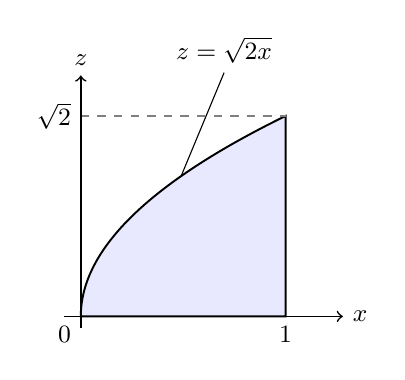
\begin{tikzpicture}[x=2.6cm,y=1.8cm]
  \path[quizregion] (0,0)--(1,0)--(1,{sqrt(2)})
    --plot[domain=1:0,samples=60,variable=\t]
      ({\t*\t},{sqrt(2)*\t})--cycle;
  \draw[dashed,gray] (0,{sqrt(2)})--(1,{sqrt(2)});
  \draw[quizaxis] (-0.08,0)--(1.28,0) node[right] {$x$};
  \draw[quizaxis] (0,-0.08)--(0,1.7) node[above] {$z$};
  \node[below left] at (0,0) {$0$};
  \node[below] at (1,0) {$1$};
  \node[left] at (0,{sqrt(2)}) {$\sqrt{2}$};
  \draw[thin] (0.49,{sqrt(2)*0.7})--(0.7,1.72)
    node[above] {$z=\sqrt{2x}$};
  %\draw[quizslice] (0.5,0)--(0.5,1);
  %\fill[blue!65!black] (0.5,0) circle (1pt) (0.5,1) circle (1pt);
\end{tikzpicture}

\textit{For each $0\leq y\leq1$, the same $xz$-cross section has
$0\leq z\leq\sqrt{2x}$.}
\end{center}

\end{enumerate}
\end{document}
